\pagebreak
\section{Messungen}%Marc 1 Seite
Für die Validierung des Gerätes wurden die beiden Layers separat ausgemessen. In den nächsten Abschnitten werden die Messungen der beiden Layer kurz erläutert und die gemessenen Abweichungen zum Erwartungswert erklärt.

\subsection*{Erster Layer}
Beim ersten Layer wurde das Netzteil, die Spannungsmessschaltung, das Relais und die Strommessschaltung, wie im Messprotokoll im Anhang ersichtlich, ausgemessen. Die Messresultate stimmten bis auf den Schaltungsteil der Strommessung mit den Erwartungswerten überein.

Bei der Strommessung wurde der Widerstand des Relais und der Sicherung vernachlässigt. Dadurch entsteht beim eingeschalteten Relais ein anderes Stromteilerverhältnis als ursprünglich angenommen. Die Abweichungen lassen sich durch einen Kompensationsfaktor ausgleichen und liegen in der akzeptierbaren Toleranz. Dies heisst, der ADC wird genügend ausgesteuert, um eine akzeptierbare Ungenauigkeit zu erlangen.

\subsection*{Zweiter Layer}
Beim zweiten Layer wurde die Abschneidspannung der Eingangsschutzschaltung, sowie die Verstärkung der Messkanäle gemessen. Diese Messungen sind in den Abbildungen \ref{fig:5A} und \ref{fig:5V} ersichtlich.

\begin{figure}[H]
\begin{center}
	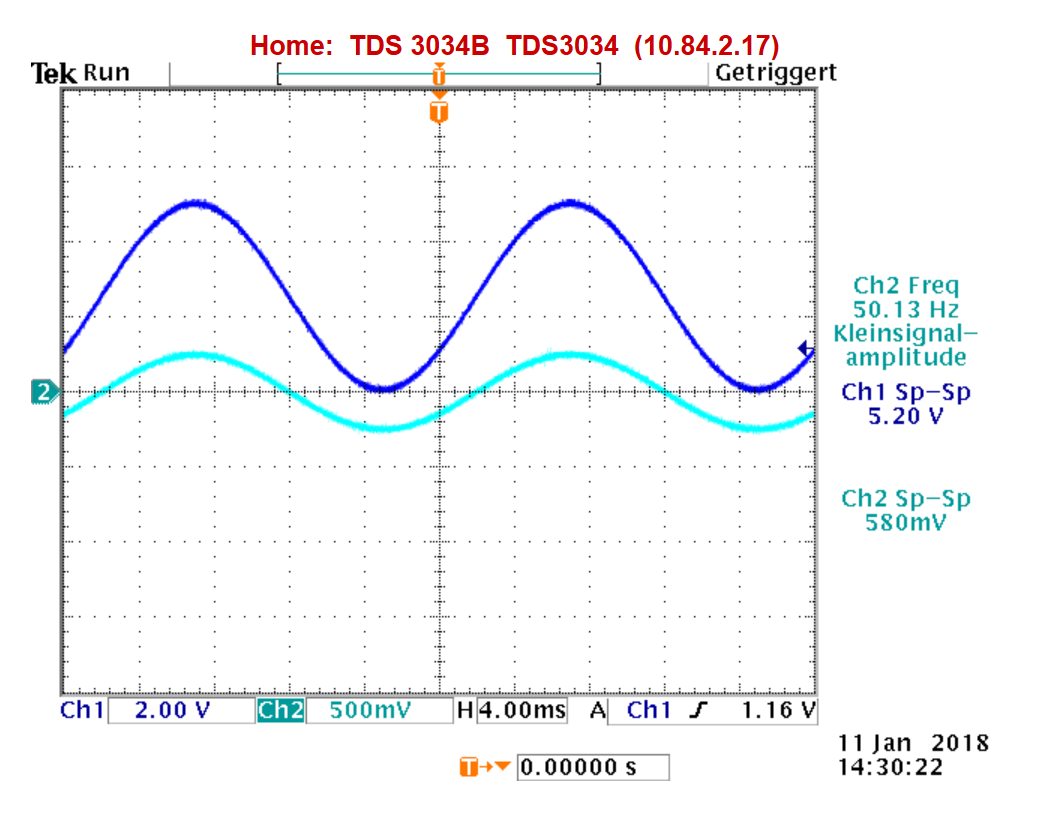
\includegraphics[width=140mm]{images/qualitatssicherung_5A_500mVpp_50Hz.png}
	\caption{Spannungsverstärkung und DC-Einkopplung des 5A Messkanals} %picture caption
	\label{fig:5A}
\end{center}
\end{figure}

In Abbildung \ref{fig:5A} ist der Ausgang (Dunkelblau) des 5A Messkanals bei einem Eingangssignal (Hellblau) von 580mV mit einer Frequenz von 50Hz abgebildet. Es ist ersichtlich, dass das Signal um den Faktor neun verstärkt und um 2.5V angehoben wird.

\begin{figure}[H]
	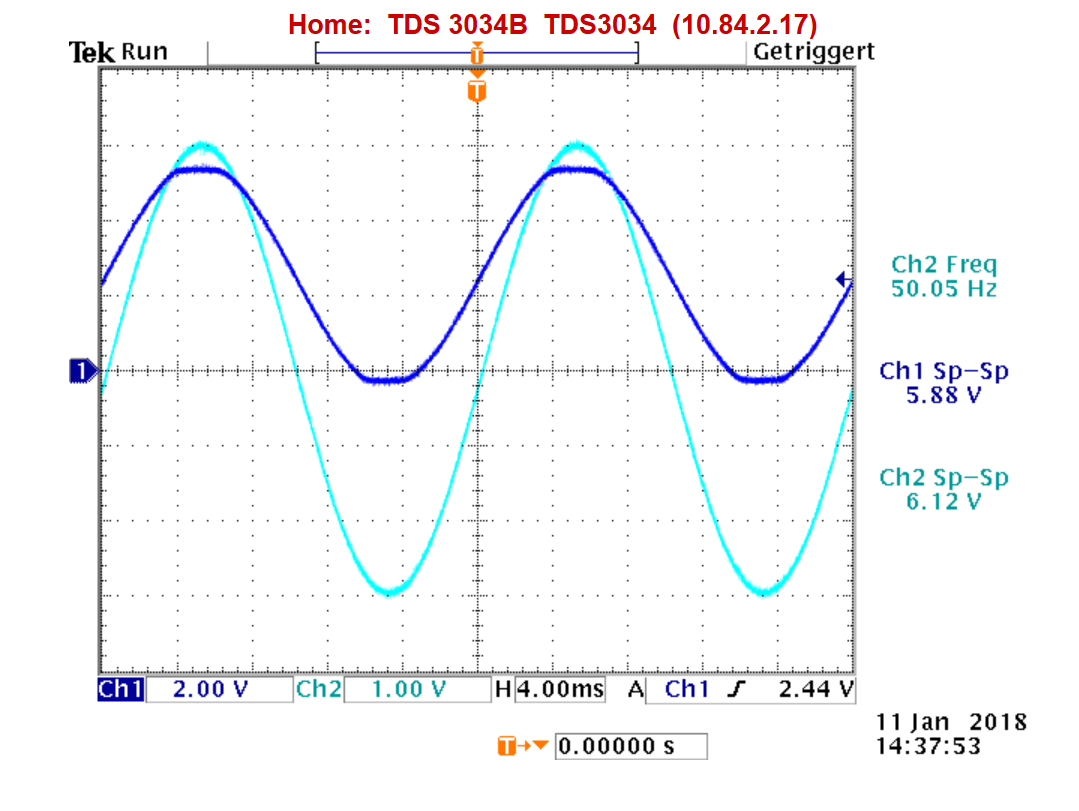
\includegraphics[width=140mm]{images/qualitatssicherung_U_5Vpp_50Hz.png}
	\caption{Messung der Eingangsschutzschaltung} %picture caption
	\label{fig:5V}
\end{figure}

In Abbildung \ref{fig:5V} ist die Funktionalität der Eingangsschutzschaltung ersichtlich. Die Spannung wird bei Eingangsspannungen unter -0.3V und über +5.3V auf die respektive Spannung begrenzt. Somit kann sichergestellt werden, dass der Eingang des ADCs nie die maximal erlaubte Eingangsspannung überschreitet. Dies ist notwendig, damit die Messbereiche nicht ausgeschaltet werden müssen, wenn sie übersteuert werden.

 